\chapter{零零阁}

在荷塘南面,西湖北面,有一座小山。西边的山头上,有一座高大的阁子,唤作零零阁。%据说是以前“零零字班”的校友捐建的,因此得名。
1970年,适逢清华园学制由6年改为5年,两个年级的学生在同一年毕业。
当时校内习惯以毕业年份来作为届号,故早一年入学的称为“零字班”,晚一年入学的便称为“零零字班”。
这座阁子,便是由零零字班的校友捐建的。
阁子有两层,有着高高的台阶,矗立在山顶上,是这一范围内最高的建筑物,可以一览原来的皇家园林的秀美景观。

之前我与C君曾在阿甘长跑时到过这个亭子。
只记得当时路过西湖附近,发现山上隐约有个亭子,便寻得路登了上去。穿过树丛,一座高大的亭子闯入眼帘。
我们正跑得气喘吁吁,这时登上二层后,阵阵凉风袭来,不胜清爽,视野也陡然开阔,一时竟有种“一览众山小”的豪迈感,仿佛胸怀也随之变得更豁达了。
我们都对当时的场面印象深刻。于是C君提议,再登一次零零阁。

然而我们都已不记得这阁子的具体位置了,只大致记得应该是在荷塘旁靠近西湖的地方,于是我们便直奔荷塘而来。
荷塘北岸一马平川,自不可能有什么山巅的阁子。而湖心岛转过一遍,也没有发现符合当时印象的双层亭阁。
于是我们向荷塘南岸寻来。

荷塘这里靠近生活区,平时晚上就有许多人来这里散步、活动,因此相比园子里其他地方,有着浓浓的市井气息,仿佛城市里的公园一般。
然而晚上出来散步的人都聚集在荷塘北岸以及湖心岛的西北角,东面和南面的人烟便十分稀少。
我们一过莲桥,就察觉这里人气淡了许多。
这时太阳已经落山,又是阴天,浓云蔽月,南岸树林相当茂密,走在幽黑的林荫小径上,一阵凉风吹过,竟觉得有一些阴冷。
越走树木越发茂密,光线也越来越暗,小径就仿佛没有出口的黑洞般,一直走不到头。这时我看到旁边有一条拐到山上的小路。
微风吹过,我微微打了个寒颤,然后指着拐出去的小路说:“那亭子应该是在山顶上,我们一直沿着湖岸走要走到什么时候,不如往这里上去找一找。”C君亦以为然,于是我们便拐到了山上去。

\begin{figure}[!h]
	\centering
	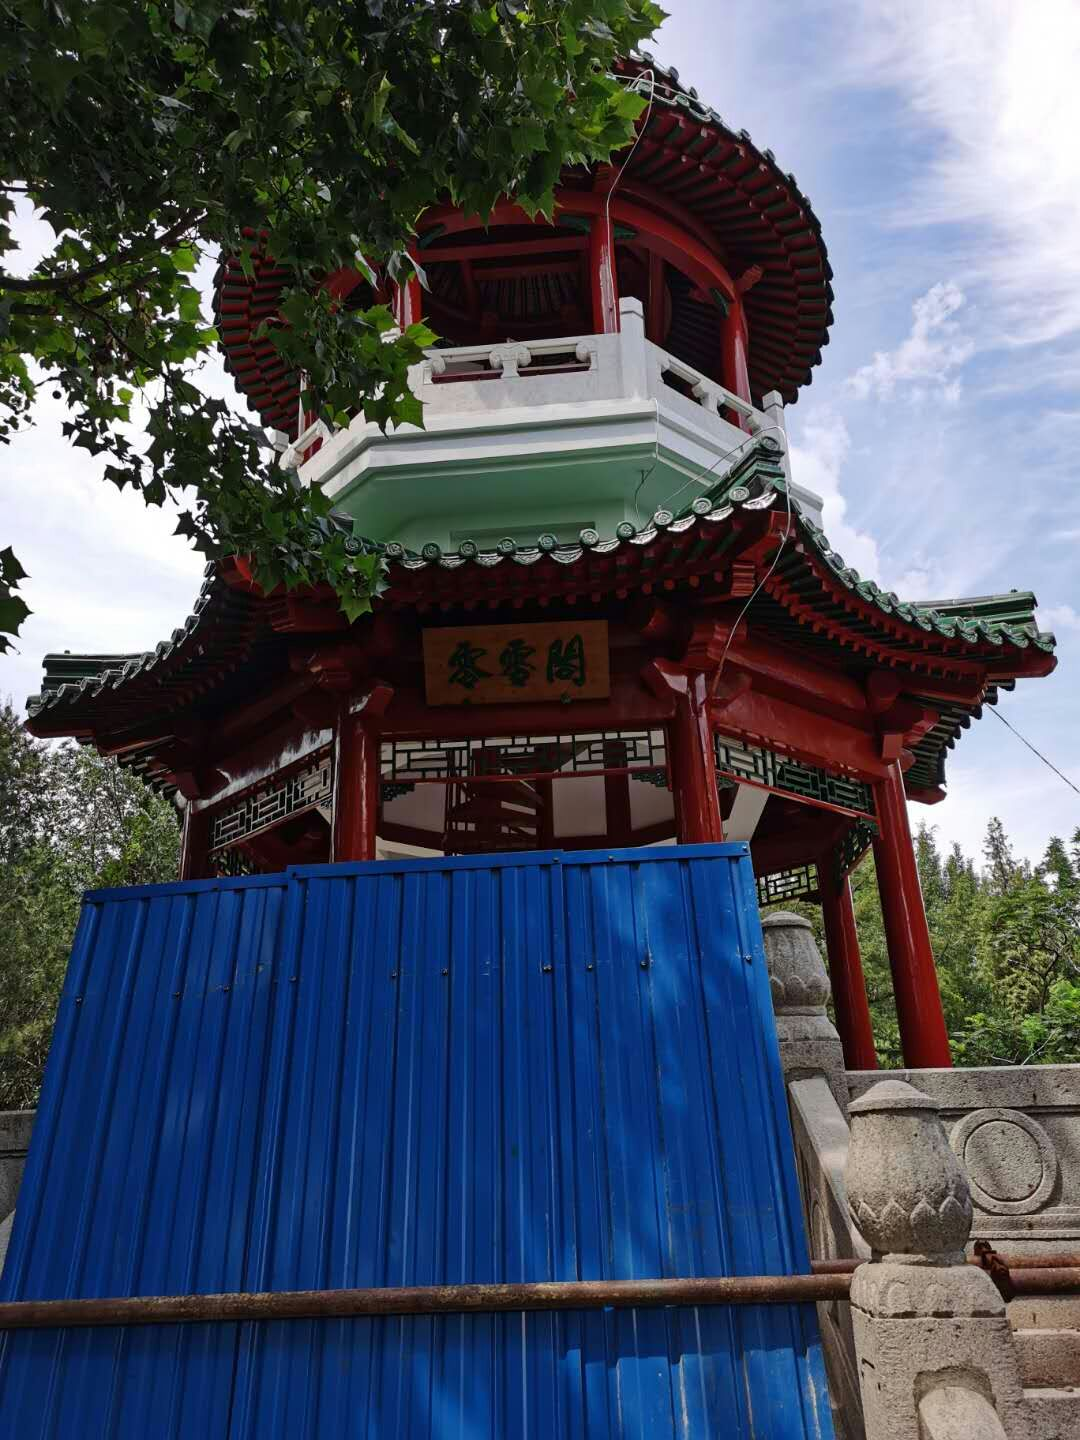
\includegraphics[width=\linewidth]{figures/零零阁.jpg}
	零零阁
\end{figure}

上山的小路坑坑洼洼的,许多铺路的石块都缺失了,表面还散布着细碎的石子,给人久未维护的感觉。
靠近山顶,树林稍稍稀疏了些,能够看到天上的阴云,也能看到前方朦胧的建筑,零零阁就在眼前了。
我们喜出望外,急忙沿着山路跑到了尽头,来到了心心念念的零零阁前,却惊讶地发现亭子已整个被围挡围住了,正在翻修中,无法再上去一瞰清华。我们大失所望,但也只好再折返下山去。
这时一阵风穿过树林,发出尖锐的啸声,我们俩不禁又打了个哆嗦,不觉间已加快了下山的脚步。
就要走出湖边的小道时,我们迎面遇到了一个满身酒气的人。或许是刚刚赴完局,打算饭后散散步,消消食,他慢悠悠地走进了林荫小道。
我们出来后,找到自己的自行车,便匆匆离去了。当晚无事。
然而第二天,就被报纸上的一条消息吓到了:“北京市某大学校内假山上发现一具无头男尸,死状凄惨,案件正在调查中。”配图正是零零阁所在的那座小山。

\vfill

\paragraph{记事}
6月23日傍晚,笔者约C君出来共游校园,途中C君提到想再上一次零零阁,于是二人往西湖与荷塘这边寻来。
寻觅良久,终于在荷塘南边的小山上找到了亭子,却发现亭子已被围起来翻修了,失望而归。
